This section provides an overview of the approach and explains how it addresses requirements R1 to R3.
A visualization of the approach is shown in Fig. \ref{fig:solution-overview}. As mentioned in \textbf{R1 Applicable on Existing Applications}, the approach shall apply to existing applications, and they should be able to support run-time state migration. For ease of enabling run-time migration for existing applications, we chose to develop the necessary library. This library shall provide an API for validation, injection, and extraction states. As stated in \textbf{Requirement R2}, the approach shall enable the ability of state specification. Thereby, modeling a run-time state as state specification is possible by the DSL, which will be integrated with the library by interfaces.

Besides libraries, our approach needs device management and device discovery, stated in \textbf{R4 Device Management}. The middleware serves as device management, allowing devices to introduce themselves and allows devices to find each other and get noticed when a device joins or leaves. These libraries can provide a point-to-point connection if devices are on the same local network. Otherwise, they use the middleware to communicate over the internet to migrate the run-time state. Since the focus of the thesis is not providing different types of communications, only one of these communication styles is implemented.

Moreover, the library need interfaces based on state specification to migrate and validate run-time states. These interfaces are converted version of state specification but provided in the same programming language of the application. They can be written manually by developers or get generated by some tools.

Furthermore, developers should write some glue code to bind the source code of the application to the library and interfaces.

\newpage
\FloatBarrier
\begin{sidewaysfigure}
\begin{figure}[H]
    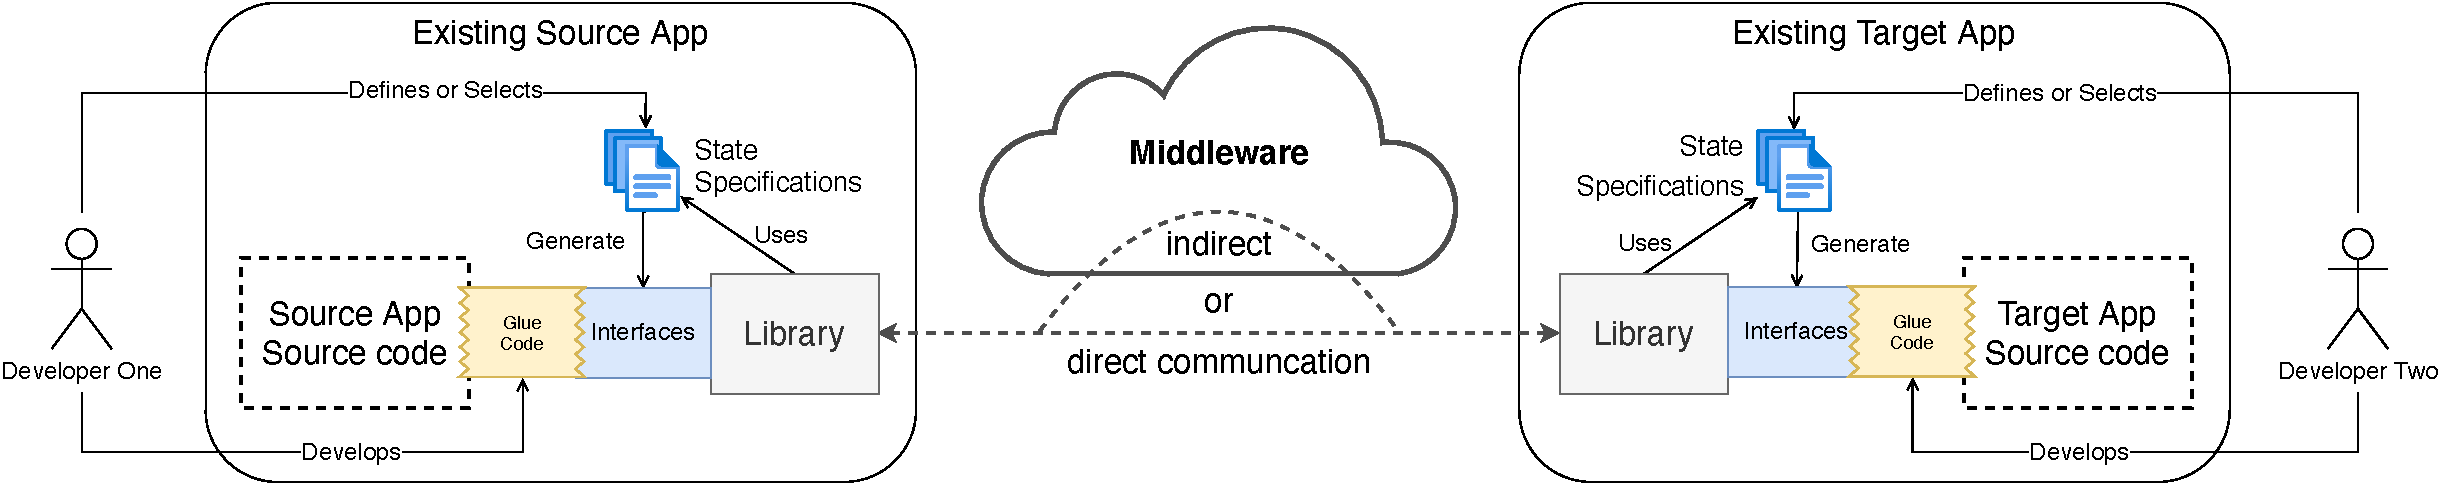
\includegraphics[width=\linewidth]{../figures/solution-overview.pdf}
    \centering
    \caption{General overview of the approach.}
    \label{fig:solution-overview}
\end{figure}
\end{sidewaysfigure}
\FloatBarrier
